\documentclass[11pt]{article}
\marginparwidth 0pt
\oddsidemargin 0pt
\evensidemargin 0pt
\marginparsep 0pt

\topmargin 0pt
\textwidth 6.5 in
\textheight 8 in

\usepackage{graphicx}
\usepackage{amssymb}
\usepackage{epstopdf}
\usepackage{amsmath}
\usepackage{color}
\newcommand{\hilight}[1]{\colorbox{yellow}{#1}}

\usepackage{bm}
%\usepackage{algorithmic}
\usepackage{url}
\usepackage[
    backend=biber,
    citestyle=ieee,
]{biblatex}
\graphicspath{ {Figures/} }
\DeclareGraphicsRule{.tif}{png}{.png}{`convert #1 `dirname #1`/`basename #1 .tif`.png}

\addbibresource{references.bib}

\title{
    A Comprehensive Report on the Mental Capabilities of Digital Monkeys
}
\author{
    Noah M. Kennedy \\[3pt]
    {\small Department of Electrical Engineering and Computer Science} \\
    {\small Milwaukee School of Engineering} \\
    {\small Milwaukee, WI, USA} \\
    {\small Email: {\tt noah.kennedy.professional@gmail.com}} \\[12pt]
\and
    Wallace O. Watler \\[3pt]
    {\small Department of Electrical Engineering and Computer Science} \\
    {\small Milwaukee School of Engineering} \\
    {\small Milwaukee, WI, USA} \\
    {\small Email: {\tt watlerathome@gmail.com}} \\[12pt]
}

\date{}

\usepackage[parfill]{parskip}

\begin{document}
    \maketitle

    \abstract
    Digital monkeys are a recently discovered species of monkey which have recently become the
subject of significant academic study due to their significant potential for use in
extraterrestrial mining operations.
Digital monkeys, like biological monkeys, can be taught to perform many advanced tasks and are
capable of complex problem solving.
In particular, they seem to exhibit advanced pathfinding and visual cognition capabilities, as well
as a sophisticated communications protocol.
Unfortunately, few researchers have previously seen fit to study in depth the mental capacities of
digital monkeys.
Previous work by this group of researchers has led to the development of a basic model of digital
monkey cognition\cite{sub_verif_plan}, however this data did not leverage significant experimental
data.
We seek to expand on that work here by leveraging data from several recent experiments to
construct a more complete picture of monkey cognition.
In this paper, we outline a novel, in-depth model of the the mental capacities of digital monkeys
across three cognitive ares: pathfinding, visual cognition, and communication, using data gained
from an ambitious set of real-world experiments we developed and performed.

    \newpage

    \tableofcontents

    \newpage

    \section{Introduction}\label{sec:introduction}
    \subsection{Problem Statement}\label{subsec:problem-statement}
The NASA RMC Lunabotics team is in need of a modular autonomous control system for their competition robot.
To meet the competition requirements, the automation system must be able to navigate from a staging area of the
competition field to a digging area and back while avoiding obstacles and without human input.

\subsection{Purpose of this Document}\label{subsec:purpose}
This report will cover the verification of our software subsystems.
A separate report has been constructed which covers the hardware aspects.
We have broken this report down by subsystem.
For each subsystem, we will provide a brief description of the system under test,
an outline and plan for the tests which were run,
and the results of those tests.

    \section{Monkey Pathfinding}\label{sec:monkey-pathfinding}
    \section{Problem Statement}\label{sec:problem-statement}
    The NASA RMC Lunabotics team is in need of a modular autonomous control system for their competition robot.
    To meet the competition requirements, the automation system must be able to navigate from a staging area of the
    competition field to a digging area and back while avoiding obstacles and without human input.

    \section{Purpose of this Document}\label{sec:purpose}
    This document follows the test/verification procedures of the software subsystems of the M.O.N.K.E.Y.\ that were
    laid out in the software subsystem testing and verification documents. Results of the verification plans are
    commented on.

    \section{Verification of the Software Subsystems}\label{sec:software-subsystems-results}

    \subsection{Monkey Pathfinding}\label{subsec:monkey-pathfinding}
    \subsubsection{Testing Suite}\label{subsubsec:testing-suite}
Table 3 below covers what software functions and components of the Nav were verified, how they were verified, and
whether each one passed.
Localization estimates are left untested until integration with the Visual Processing Software Subsystem since they
require both subsystems to work together.
\begin{center}
    \begin{tabular}{ |c|c|c|c| }
        Name & Objectives & Definition & Results \\
        A* & Correctness - Is the algorithm implemented in a sound manner? & Unit tests & Pass \\
        Nav & Safety - Does it avoid steep (>20° incline) slopes? Adherence to the supplied parameters - Start and end position and orientation, minimum turn radius Length - Does it take a reasonable path, not looping or backtracking? & Unit tests & Pass \\
        Mesh to Grid & Faithfulness - Does the grid representation closely match the physical terrain? & Human-reviewed & Pass
    \end{tabular}
\end{center}
\subsubsection{Changes from Previous Verification Plan}\label{subsubsec:changes-to-plan}
Previously, the gradient grid obtained from the triangle mesh did not accurately reflect the physical environment in
some cases.
The biggest issue was that overhangs with vertical faces, when flattened to 2D, appeared as a massive spike in the
terrain heightmap.
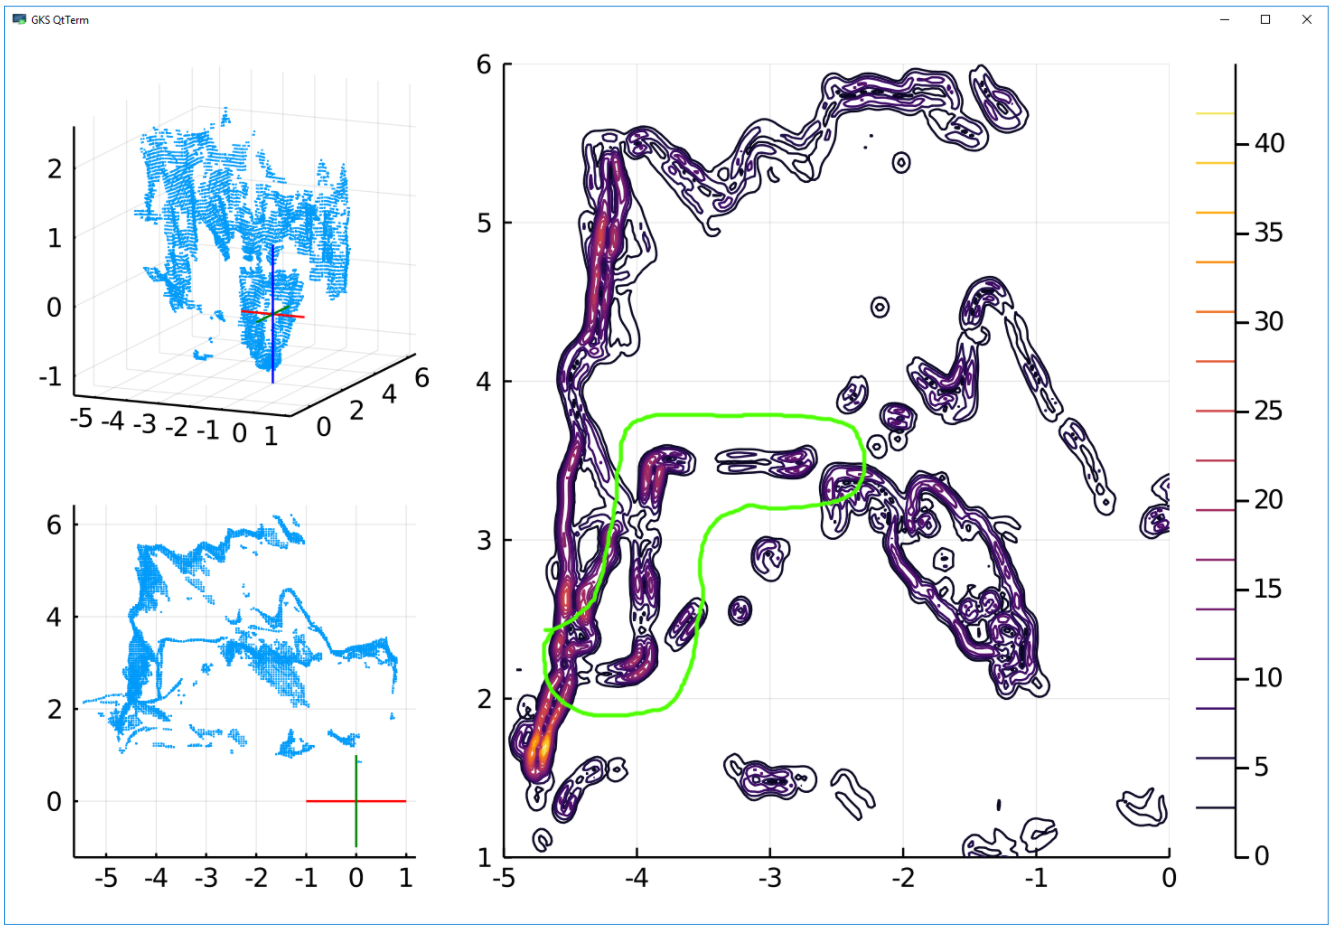
\includegraphics{mesh-to-grid-old}


    \subsection{Monkey Communication}\label{subsec:monkey-communication}
    \subsubsection{Subsystem Overview}
The communications subsystem consists of several network Application Programming Interface (API)
endpoints.
These endpoints cover domains such as serving camera feeds, operating a flight director which
provides continuous, real-time instructions for robot operation, creating flight plans,
and obtaining localization estimates and maps of the field.

\subsubsection{Test Plan}
There were two methods of verification which our plan called for.

The first method of verification was a comprehensive endpoint unit test suite.
Each endpoint was hit by a test client to confirm that the endpoint was showing data in the correct
format.
This was done using the unit testing facilities provided by the standard rust tooling, as well as
asynchronous HTTP clients.
Code coverage was recorded and monitored on within the communications codebase using the
Tarpaulin\cite{tarpaulin} tool to ensure that each endpoint was being hit.

The second method of verification was a manual test of network bandwidth utilization while
streaming video feeds from our cameras.
This test was conducted by starting a camera stream at 15 frames per second at a resolution of
1280x720p while using Wireshark\cite{wireshark} to capture packets and plot the bandwidth usage of
the program.
The test would be successful if the bandwidth utilization was under 2,000 kilobits per second,
although a much lower value of under 1,000 was targeted as an informal goal.

\subsubsection{Test Results}


    \subsection{Monkey Target Detection}\label{subsec:monkey-target-detection}
    \subsubsection{Overview}
During the NASA Lunabotics competition, visual fiducial markers may be placed above the collection
bin in order to assist the robot in finding and navigating to the bin.
The visual tracking subsystem implements detection and range finding for several fiducial markers
at a time.
The AprilTag system of fiducial markers was chosen for the implementation of the visual tracking
subsystem, specifically the 36h11 family of tags, due to its robustness even at long distances, as
well as a widespread userbase in robotics and computer vision applications.
The StereoLabs ZED 2 stereo camera, which is used to collect 3D point cloud data for the pathfinding
subsystem, is used in conjunction with the OpenCV computer vision API to detect the AprilTag targets.
A single camera view is used to detect the tags, and then stereo vision is used to determine the
distance to the tag once it has been located.
\begin{figure}[htbp]
    \centering
    
\includegraphics[width=50mm]{april}
    \caption{
        Example of an AprilTag fiducial target
    }\label{fig:april}
\end{figure}

\begin{figure}[htbp]
    \centering
    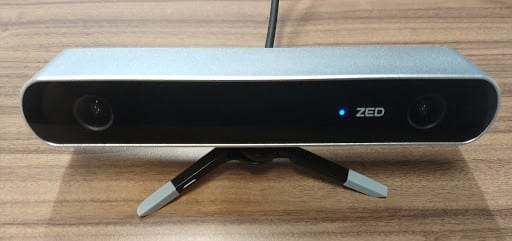
\includegraphics[width=50mm]{zed}
    \caption{
        The ZED 2 stereo camera
    }\label{fig:zed}
\end{figure}

\newpage

\subsubsection{Test Plan}
The visual tracking subsystem is verified through manual testing.
Testing is conducted by setting up a computer with the ZED 2 plugged in and placing AprilTag markers,
either printed or on a computer screen, in front of the camera.
The software should detect any targets in view and determine the distance to any target placed
greater than 50cm away from he camera (as the device cannot accurately measure range within 50cm).
For thorough results, multiple targets should be tested at several different ranges and angles,
and in different lighting conditions.
A tape measure can be used to verify the accuracy of the range measurements.

\subsubsection{Test Results}
The vision subsystem was able to successfully identify multiple targets and accurately measure the
distance to within several cm and at very wide viewing angles.
In good lighting conditions, the device was able to detect targets at a range of up to 2.6m,
while in very poor lighting it could detect targets up to 2m away.
Due to USB bandwidth limitations of the computer used in testing, the test was run at a resolution
of only 1344x376.
With a faster USB port, the ZED camera can run at resolutions of up to 2K,
which should significantly increase the target detection range.

\newpage

\begin{figure}[!htbp]
    \centering
    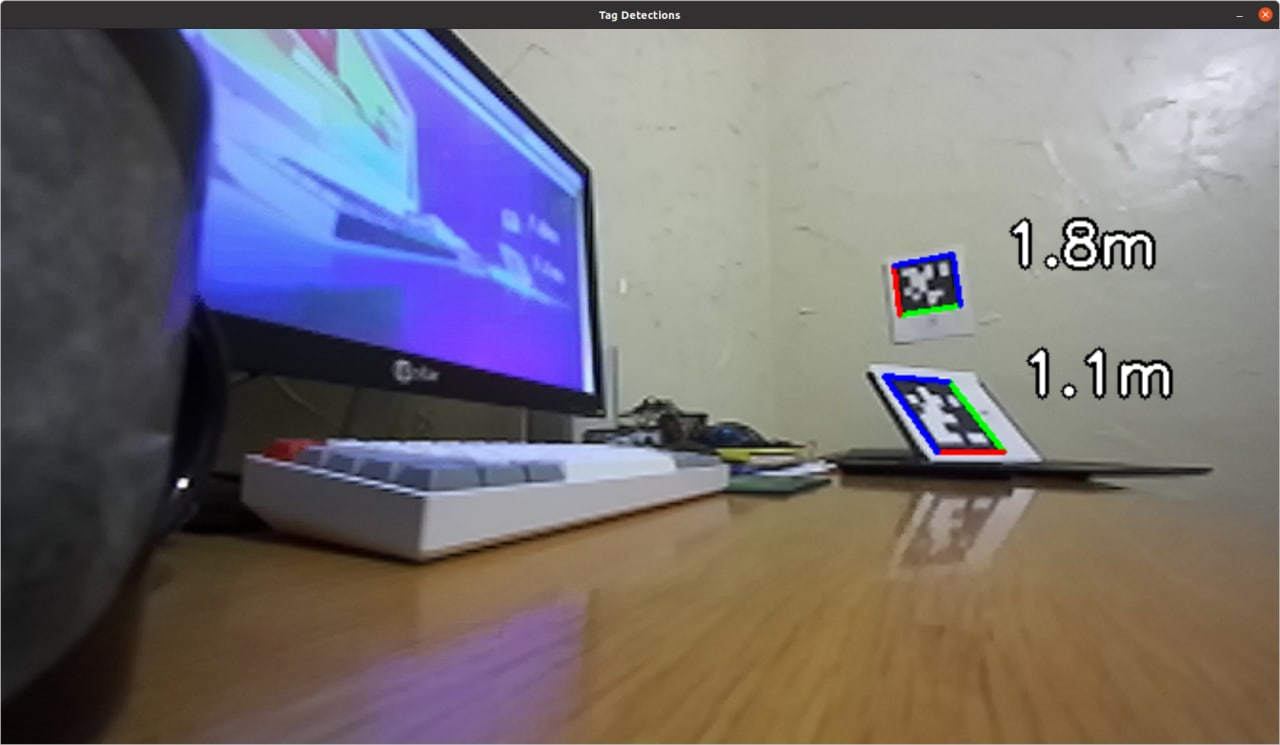
\includegraphics[width=150mm]{glt}
    \caption{
        Test in good lighting conditions
    }\label{fig:glt}
\end{figure}

\begin{figure}[!htpb]
    \centering
    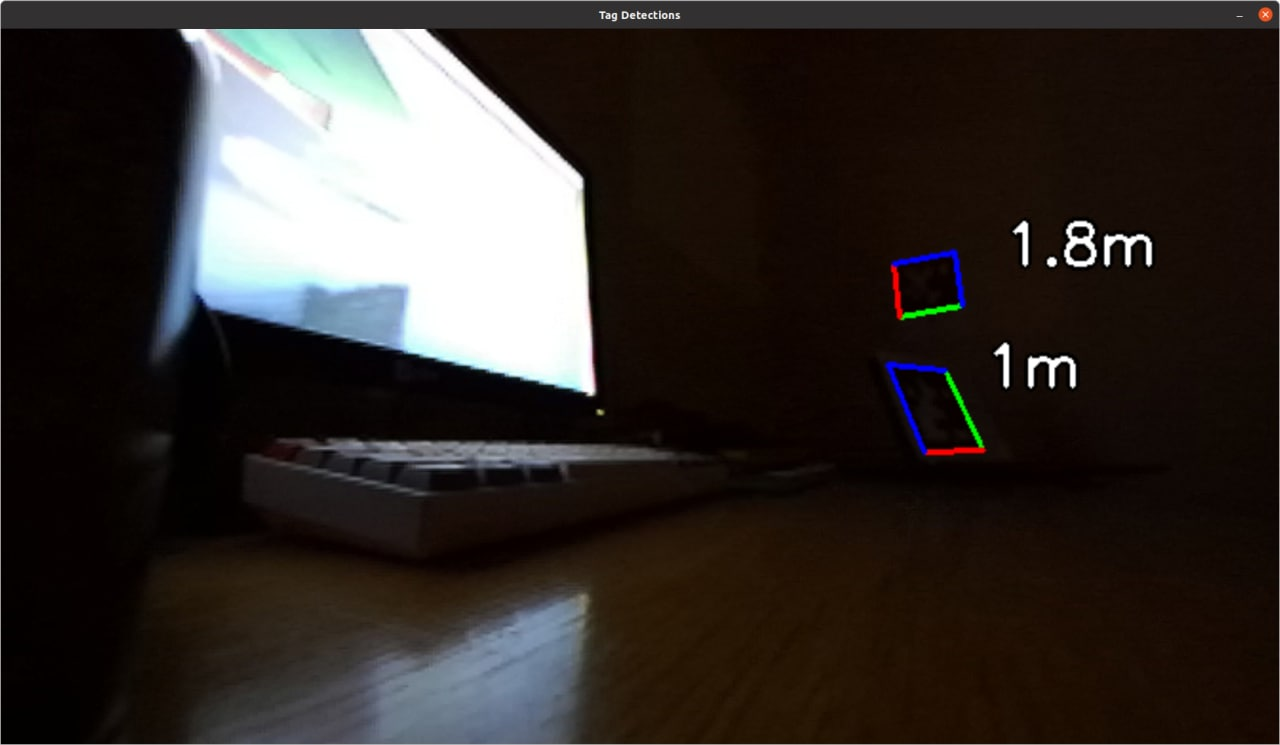
\includegraphics[width=150mm]{plt}
    \caption{
        Test in poor lighting conditions
    }\label{fig:plt}
\end{figure}
\newpage

    \section*{Appendix}\label{sec:appendix}

    \pagebreak

    \printbibliography
\end{document}
